\subsection{Instalasi Pip}
Pip merupakan modul atau paket yang harus kita miliki apabila kita menggunakan bahasa pemrograman python. Pip digunakan untuk menginstal package-package python yang akan kita gunakan dalam pembuatan kode program.
Cara melakukan instalasi pip pada anaconda CLI: 
\begin{enumerate}
\item buka anaconda prompt (Start -> Anaconda Prompt)
\item ketikkan conda install -c anaconda pip seperti pada gambar \ref{Figureanaconda10}.
\begin{figure}[H]
    \centering
    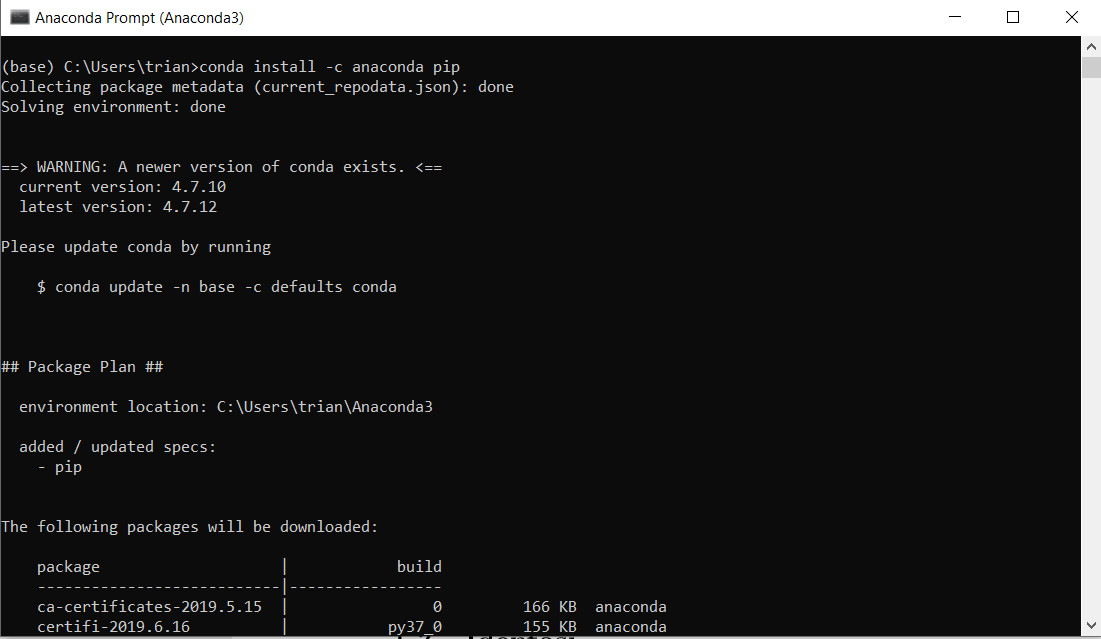
\includegraphics[scale=0.4]{figures/installpip}
    \caption{\textit{Install pip}}
    \label{Figureanaconda10}
\end{figure}
\item ketik y, lalu enter. Tunggu hingga proses instalasi selesai seperti pada gambar \ref{Figureanaconda11}.
\begin{figure}[H]
    \centering
    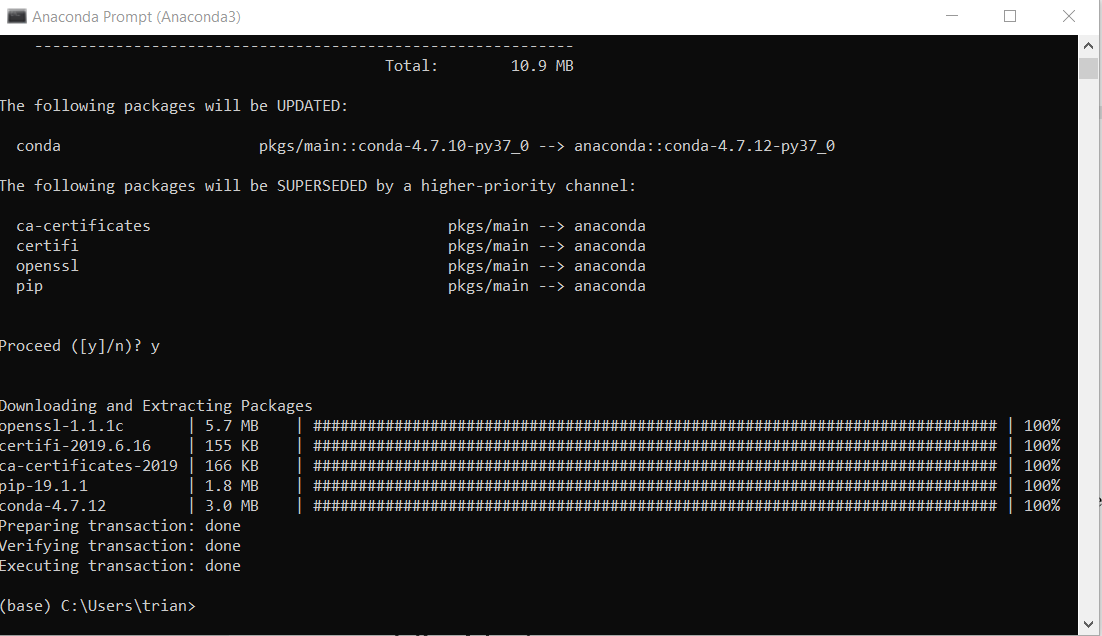
\includegraphics[scale=0.4]{figures/pipselesai}
    \caption{\textit{Install pip Selesai}}
    \label{Figureanaconda11}
\end{figure}
\item jika telah selesai, lakukan pengecekan versi pip dengan mengetikkan pip -V seperti pada gambar \ref{Figureanaconda12}.
\begin{figure}[H]
    \centering
    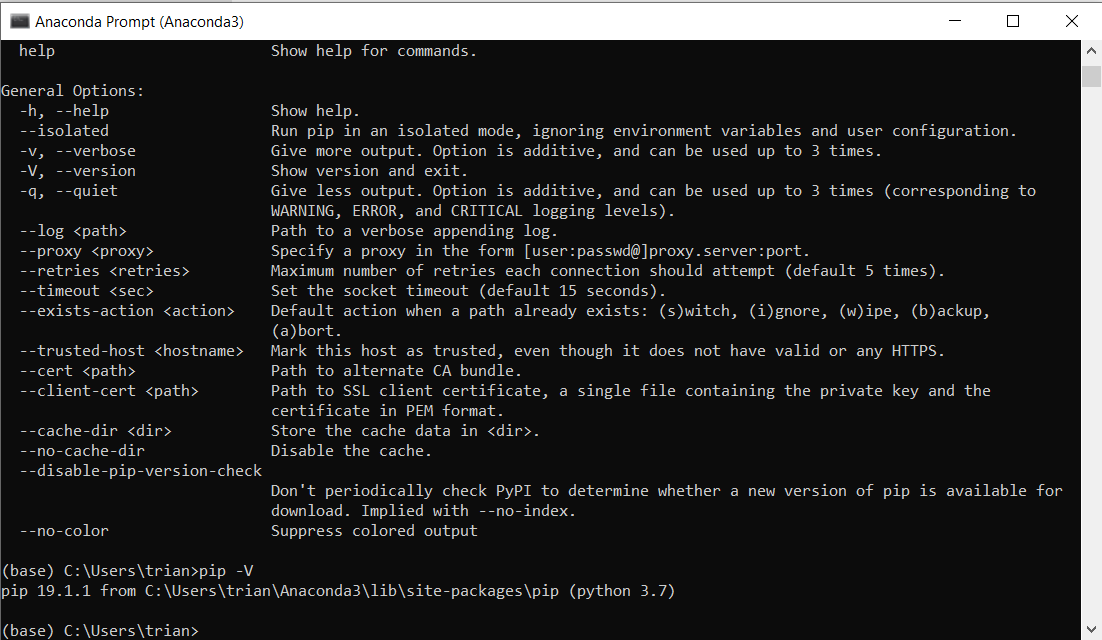
\includegraphics[scale=0.4]{figures/pipversion}
    \caption{\textit{Melihat Versi pip}}
    \label{Figureanaconda12}
\end{figure}

\end{enumerate}

\subsection{Command Line Interface/Interpreter}
Command line interpreter atau yang biasa teman-teman ketahui sebagai command prompt memungkinkan kita untuk menuliskan baris perintah yang akan dijalankan oleh komputer. Command line interpreter hanya berupa script atau tulisan kode program, berbeda dengan grapich user interface atau GUI yang memungkinkan kita memerintahkan sesuatu kepada komputer dengan hanya menggunakan tombol-tombol dan tampilan yang mudah dipahami.
Cara menjalankan program python pada CLI:
\begin{enumerate}
\item Buka command prompt lalu ketikkan python seperti pada gambar \ref{CLI}.
\item Buatlah perintah print, input, perkalian, dan pembagian seperti pada gambar \ref{CLI}.
\item Bisa juga menjalankan file .py yang telah dibuat di IDE dengan cara python namafile.py, lalu klik enter seperti pada gambar \ref{CLI}.
\begin{figure}[H]
    \centering
    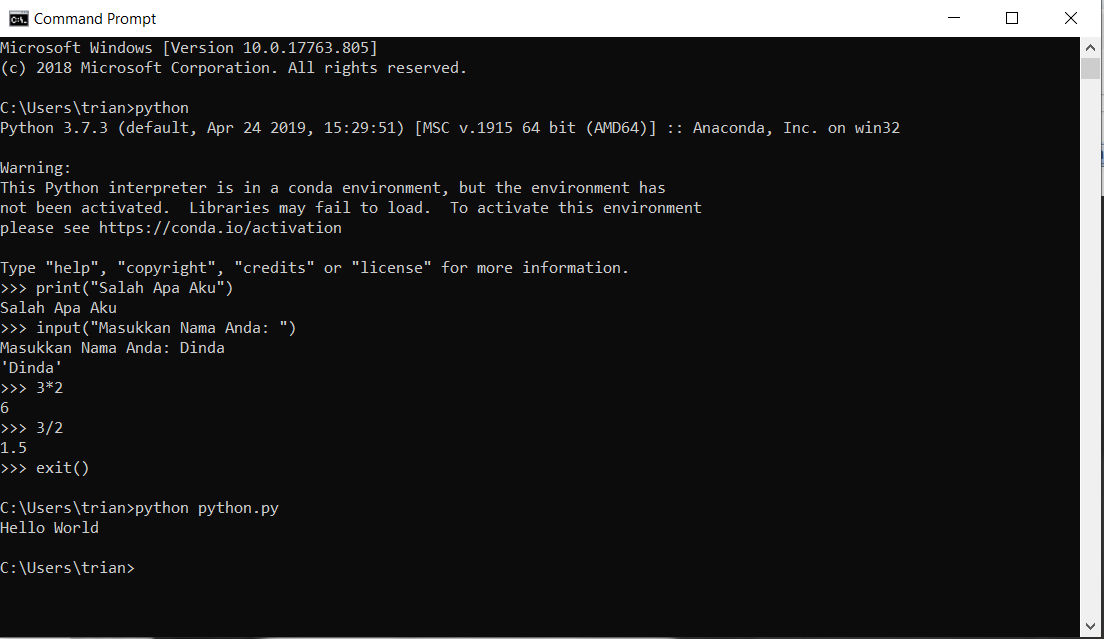
\includegraphics[scale=0.4]{figures/cli}
    \caption{\textit{CLI in Command Prompt}}
    \label{CLI}
\end{figure}
\end{enumerate}